\section{Stochastic Optimization}

The goal is to $\min_{x \in X} F(x) = \frac{1}{n}\sum_{i=1}^n f_i(x)$, or more generally, $\min_{x \in X} F(x) = \E_\xi (f(x, \xi))$. For large $n$, computing the full gradient is expensive. For unknown $P(\xi)$, the gradient is intractable.

\textbf{Stochastic gradient quality for smooth functions}: (12.12) let $F(x)=\frac{1}{n}\sum_{i=1}^n f_i(x)$, where $f_i$ is $L_i$-smooth and convex, and $F$ has a global minimum $x^*$. Let $L_{\text{max}} = \max_i\{L_i\}$, then for any $x$ we have $\frac{1}{n}\sum_{i=1}^n \|\nabla f_i(x) - \nabla f_i(x^*)\|^2 \le 2L_{\text{max}}(F(x) - F(x^*))$. Proof: define $g_i(x) = f_i(x) - f_i(x^*) - \nabla f_i(x^*)^\top (x-x^*)$. Thus, $g_i(x)\ge 0$, and is convex and $L_i$-smooth. By sufficient decrease, we have $0\le g_i(x - \frac{1}{L_i}\nabla g_i(x)) \le g_i(x) - \frac{1}{2L_i}\|\nabla g_i(x)\|^2$. Thus, $g_i(x) \ge \frac{1}{2L_{\text{max}}}\|\nabla g_i(x)\|^2$. Expanding this by definition, summing over $i$, and using $\nabla F(x^*)=0$ yields the result. Note that the proof works for the general $F(x) = \E(x,\xi)$.

\textbf{Stochastic gradient descent}: do $x_{t+1} = \Pi_X (x_t - \gamma_t \nabla f(x_t, \xi_t))$. In the finite-sum problem, this is $x_{t+1} = \Pi_X(x_t - \gamma_t \nabla f_{i_t}(x_t))$, where $i_t$ is sampled uniformly at random. Thus, the \emph{gradient is unbiased}: $\E_{i_t} (\nabla f_{i_t} (x_t) \mid x_t) = \sum_i \frac{1}{n} \nabla f_i (x_t) = \nabla F(x_t)$, or $\E(\nabla f(x_t, \xi_t) \mid \xi_{[t-1]}) = \nabla F(x_t)$. The step size should diminish, i.e., $\gamma_t \rightarrow 0$, to ensure convergence, as the stochastic gradient does not necessarily equal to zero at the optima.

\textbf{Analysis}:
\begin{enumerate}
    \item \textbf{Strongly convex functions}: (12.3) assume $F(x)$ is $\mu$-strongly convex and $\E(\|\nabla f(x, \xi)\|^2) \le B^2$ for any $x \in X$. With $\gamma_t = \gamma / t$ for $\gamma > \frac{1}{2\mu}$, SGD satisfies $\E(\|x_t - x^*\|^2) \le \frac{C(\gamma)}{t}$, where $C(\gamma) = \max \{\frac{\gamma^2 B^2}{2\mu\gamma -1}, \|x_1 - x^*\|^2\}$. Proof: by projection inequality, $\|x_{t+1} - x^*\|^2 \le \|x_t - \gamma_t \nabla f(x_t, \xi_t) - x^*\|^2 = \|x_t - x^*\|^2 - 2\gamma_t \langle \nabla f(x_t, \xi_t), x_t - x^* \rangle + \gamma_t^2 \|\nabla f(x_t, \xi_t)\|^2$. Taking expectation, we have $\E(\|x_{t+1} - x^*\|^2) \le \E(\|x_t - x^*\|^2) - 2\gamma_t \E(\langle \nabla f(x_t, \xi_t), x_t - x^*\rangle) + \gamma_t^2 B^2$. Note that  $\E(\langle \nabla f(x_t, \xi_t), x_t - x^*\rangle) = \E\left[\E(\langle\nabla f(x_t, \xi_t), x_t-x^*\rangle \mid \xi_{[t-1]})\right] = \E(\langle \nabla F(x_t), x_t - x^*\rangle)$. By strong convexity, $\langle \nabla F(x_t), x_t - x^* \rangle \ge \mu \|x_t - x^*\|^2$, thus $\E(\|x_{t+1} - x^*\|^2) \le (1-2\mu \gamma_t)\E(\|x_t - x^*\|^2) + \gamma_t^2 B^2$. The result follows by induction.
    \item \textbf{Convex functions}: (12.4) let $F$ be convex and $\E(\|\nabla f(x, \xi)\|^2) \le B^2$ for any $x \in X$. SGD satisfies $\E(F(\hat{x_T}) - F(x^*)) \le \frac{R^2 + B^2 \sum_{t=1}^T \gamma_t^2}{2\sum_{t=1}^T \gamma_t}$ for $\hat{x_T} = \frac{\sum_{t=1}^T \gamma_t x_t}{\sum_{t=1}^T \gamma_t}$. Proof: use $\langle \nabla F(x_t), x_t - x^* \rangle \ge F(x_t) - F(x^*)$ in the proof of (12.3) gives $\gamma_t \E(F(x_t) - F(x^*)) \le \frac{1}{2}\E(\|x_t -x^*\|^2) - \frac{1}{2}\E(\|x_{t+1} - x^*\|^2) + \frac{1}{2}\gamma_t^2 B^2$. The result follows by recursion and convexity.
    \item \textbf{Strongly convex and smooth functions, constant step size}: (12.5) assume $F(x)$ is both $\mu$-strongly convex and $L$-smooth, and $\E(\|\nabla f(x, \xi)\|^2) \le \sigma^2 + c\|\nabla F(x)\|^2$. Then, with $\gamma_t = \gamma \le \frac{1}{Lc}$, $\E(F(x_t) - F(x^*)) \le \frac{\gamma L \sigma^2}{2\mu} + (1-\gamma \mu)^{t-1}(F(x_1) - F(x^*))$.
    \item \textbf{Non-convex but smooth function}: (12.8) assume $F(x) = \E(f(x, \xi))$ is $L$-smooth and $\E(\|\nabla f(x, \xi) - \nabla F(x)\|^2) \le \sigma^2$, then with $\gamma_t = \min\{1/L, \frac{\gamma}{\sigma\sqrt{T}}\}$, SGD achieves $\E(\|\nabla F(\hat{x}_T)\|^2) \le \frac{\sigma}{T}\left(2(F(x_1) - F(x^*))/\gamma + L\gamma\right)$, where $\hat{x}_T$ is selected uniformly at random from $\{x_1, \dots, x_T\}$. Proof: by $L$-smoothness and $x_{t+1}=x_t-\gamma_t \nabla f(x_t, \xi_t)$, we have $\E(F(x_{t+1}) - F(x_t)) \le \E(\nabla F(x_t)^\top (x_{t+1} - x_t) + \frac{L}{2}\|x_{t+1} - x_t\|^2) \le \E(-\gamma_t \nabla F(x_t)^\top \nabla f(x_t, \xi_t) + \frac{L\gamma_t^2}{2}\|\nabla f(x_t, \xi_t)\|)$. Using $\E(\nabla f(x_t, \xi_t) \mid x_t) = \nabla F(x_t)$ and $\E(\|\nabla f(x_t, \xi_t)\|^2 \mid x_t) \le \sigma^2 + \|\nabla F(x_t)\|^2$, this implies $\E(F(x_{t+1}) - F(x_t)) \le -\frac{\gamma_t}{2}\E(\|\nabla F(x_t)\|^2) + \frac{L\sigma^2\gamma_t^2}{2}$ since $\gamma_t \le 1/L$. The result follows by induction.
\end{enumerate}

\textbf{Variants of SGD}
\begin{enumerate}
    \item \textbf{AdaGrad}: do $v_t = v_{t-1} + \nabla f(x_t, \xi_t)^{\odot 2}$ and $x_{t+1} = x_t - \frac{\gamma_0}{\epsilon+\sqrt{v_t}} \odot \nabla f(x_t, \xi_t)$, where $\odot$ means element-wise operation. Idea: adjust learning rate for different coordinate, use smaller step-size for mostly updates coordinates. Problem: learning rate is adjusted too aggressively and becomes too small at a later stage.
    \item \textbf{RMSProp}: do $v_t = \beta v_{t-1} + (1-\beta)\nabla f(x_t, \xi_t)^{\odot 2}$ and $x_{t+1} = x_t - \frac{\gamma_0}{\epsilon+\sqrt{v_t}} \odot \nabla f(x_t, \xi_t)$. Idea: use a moving aqerage as the discount factor so that the discount factor does not grow too fast. $\beta$ is chosen close to 1.
    \item \textbf{Adam}: do $v_t = \beta_2 v_{t-1}+(1-\beta_2)\nabla f(x_t, \xi_t)^{\odot 2}$, $m_t = \beta_1 m_{t-1} + (1-\beta_1)\nabla f(x_t, \xi_t)$ and $x_{t+1} = x_t - \frac{\gamma_0}{\epsilon + \sqrt{v_t / (1-\beta_2^t)}}\odot \frac{m_t}{1-\beta_1^t}$. Idea: combining momentum with learning rate adjustment. $\beta_1$ and $\beta_2$ are chosen close to 1.
\end{enumerate}

\textbf{Variance Reduction Technique}: the convergence guarantee of SGD with constant step size depends on the variance of the gradient. Reducing its variance makes it converge to a nearer point to the optimal.
\begin{enumerate}
    \item \textbf{Mini-batch}: use a mini-batch to estimate gradient, i.e., $\nabla f(x_t, \xi_t) = \frac{1}{b}\sum_{i=1}^b \nabla f(x_t, \xi_{t, i})$.
    \item \textbf{Momentum}: do $x_{t+1}=x_t - \gamma_t \hat{m}_t$, where $\hat{m}_t = c\sum_{\tau=1}^t \alpha^{t-\tau} \nabla f_{i_\tau}(x_\tau)$ is the weighted average of the past stochastic gradients.
    \item \textbf{Control variate}: assume we want to estimate $\theta=\E X$, and we know a random variable $Y$ that is highly correlated with $X$ and $\E Y$ can be computed easily. Then $\hat{\theta}_\alpha := \alpha(X-Y)+\E Y$ has smaller bias and larger variance when $\alpha$ increases from 0 to 1. When $\alpha=0$ it has zero variance and when $\alpha=1$ it has zero bias.
\end{enumerate}

\textbf{Stochastic variance-reduced algorithms}:
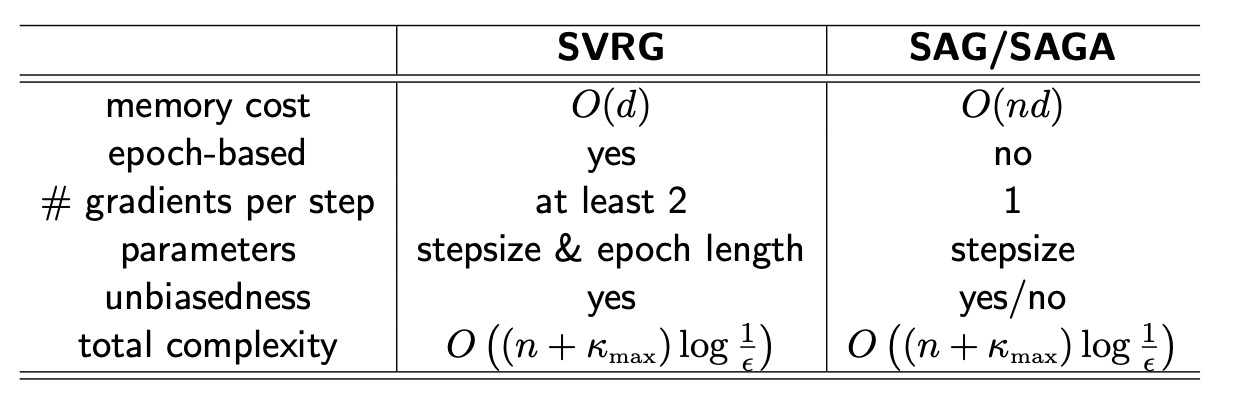
\includegraphics[width=\linewidth]{imgs/SVRG.jpg}
\begin{enumerate}
    \item \textbf{Stochastic average gradient (SAG)}: use average of the past gradient as an estimate of the full gradient: $g_t = \frac{1}{n}\sum_{i=1}^n v_i^t$, where $v_i^t = \nabla f_{i_t}(x_t)$ for $i=i_t$ and $v_i^t=v_i^{t-1}$ otherwise. Equivalently, $g_t = g_{t-1} + \frac{1}{n}(\nabla f_{i_t}(x_t) - v_{i_t}^{t-1})$. This means SAG is as cheap as SGD. It has convergence rate linear in $\log{1/\epsilon}$ for strongly convex and smooth functions.
    \item \textbf{SAGA}: use $g_t = \nabla f_{i_t}(x_t) - v_{i_t}^{t-1} + \frac{1}{n}\sum_{i=1}^n v_i^{t-1}$ to make it unbiased. It has the same rate as SAG.
    \item \textbf{Stochastic variance-reduced gradient (SVRG)}: use a fixed reference point to estimate the gradient: $g_t = \nabla f_{i_t}(x_{t}) - \nabla f_{i_t}(\tilde{x}) + \nabla F(\tilde{x})$ and $x_{t+1} = x_{t} - \eta g_t$, where the reference point $\tilde{x}_t$ is updated only once a while. Idea: $\E(\|g_t - \nabla F(x_t)\|^2) \le \E(\|\nabla f_{i_t}(x_t) - \nabla f_{i_t}(\tilde{x})\|^2) \le L_{\text{max}}^2\|x_t - \tilde{x}\|^2$, so the variance is bounded by how close $x_t$ is to $\tilde{x}$. Typical choice of $\tilde{x}$: each epoch $s$ consists of $m$ update, then use $\tilde{x}^s = \frac{1}{m}\sum_i x_t$ as the reference point of next epoch.
\end{enumerate}

\textbf{Convergence of SVRG}: (12.11) assume $f_i(x)$ is convex and $L$-smooth and $F(x)=\frac{1}{n}\sum_{i=1}^n f_i(x)$ is $\mu$-strongly convex. Let $x^*=\argmin_x F(x)$. For large $m$ and $\eta < \frac{1}{2L}$, and $\rho:=\frac{1}{\mu\eta(1-2L\eta)m}+\frac{2L\eta}{1-2L\eta} < 1$, we have $\E(F(\tilde{x}^s) - F(x^*)) \le \rho^s(F(\tilde{x}^0) - F(x^*))$. Proof: by $\|a+b\|^2\le 2\|a\|^2+2\|b\|^2$, we have $\E(\|g_t\|^2) \le 2\E(\|\nabla f_{i_t}(x_{t}) - \nabla f_{i_t}(x^*)\|^2) + 2\E(\|\nabla f_{i_t}(\tilde{x}) - \nabla f_{i_t}(x^*) - \nabla F(\tilde{x}^*)\|^2)$. Notice $\E(\|\nabla f_{i_t}(\tilde{x}) - \nabla f_{i_t}(x^*) - \nabla F(\tilde{x}^*)\|^2) = \E(\|\nabla f_{i_t}(\tilde{x}) - \nabla f_{i_t}(x^*)\|^2)$ and use lemma 12.12, we have $\E(\|g_t\|^2) \le 4L(F(x_{t}) - F(x^*) + F(\tilde{x}) - F(x^*))$. Therefore, $\E(\|x_{t+1}-x^*\|^2) = \|x_t - x^*\|^2 - 2\eta(x_t - x^*)^\top \E(g_t) + \eta^2\E(\|g_t\|^2) \le \|x_t - x^*\|^2 -2\eta(1-2L\eta)(F(x_t) - F(x^*)) + 4L\eta^2(F(\tilde{x}) - F(x^*))$. By convexity, we have $-\sum_{i=1}^m \E(F(x_{t} - F(x^*))) \le -m \E(F(\tilde{x}) - F(x^*))$. In addition, by strong convexity, we have $\E(\|\tilde{x} - x^*\|^2) \le \frac{2}{\mu}\E(F(\tilde{x}) - F(x^*))$. Combining these three gives the desired result. Set $\eta=O(1/L)$ and $m=O(L/\mu)$ makes $\rho \in (0, 0.5)$. Thus, the convergence is linear in $O(\log(1/\epsilon))$.

Other methods: 

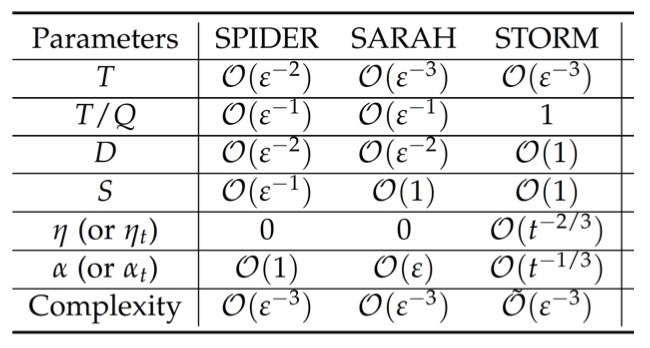
\includegraphics[width=\linewidth]{imgs/SGD-var.jpg}